% This work is made available under the terms of the
% Creative Commons Attribution-ShareAlike 4.0 license,
% http://creativecommons.org/licenses/by-sa/4.0/.
%
% Version: $Revision$

\chapter{Visualization}

\section{Preview browser}
The WEKA module comes with custom viewers for serialized files. Apart from the
default view (Figure \ref{previewbrowser-default}), you can also view the
trees (Figure \ref{previewbrowser-tree}) and graphs (Figure \ref{previewbrowser-graph})
that some classifiers generate.

\begin{figure}[htb]
  \centering
  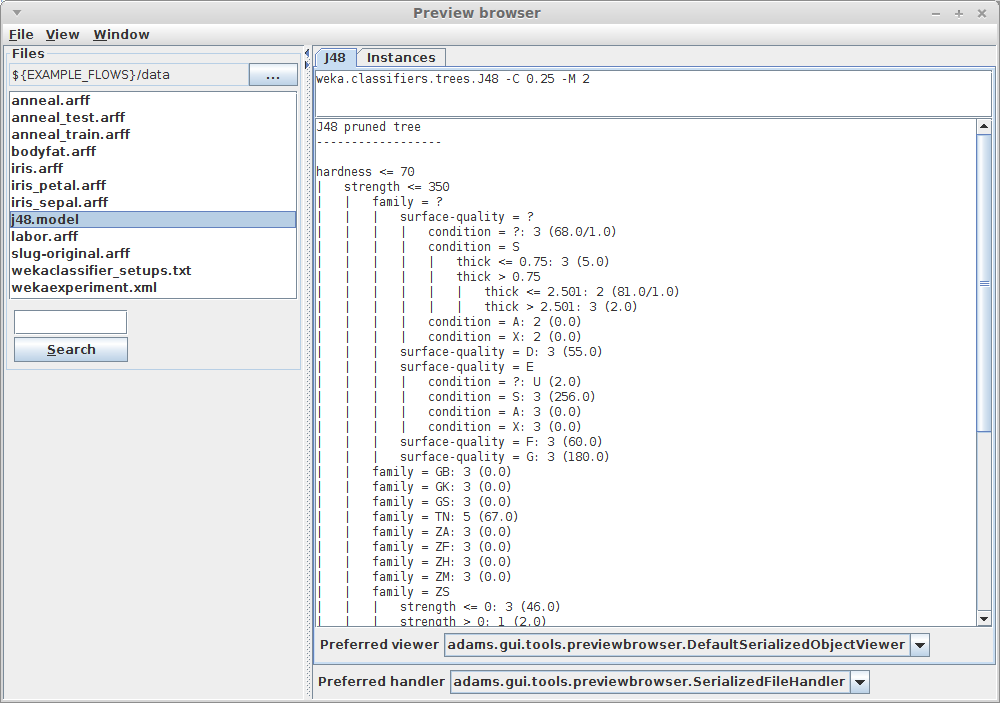
\includegraphics[width=10.0cm]{images/previewbrowser-default.png}
  \caption{Default preview for classifier.}
  \label{previewbrowser-default}
\end{figure}

\begin{figure}[htb]
  \centering
  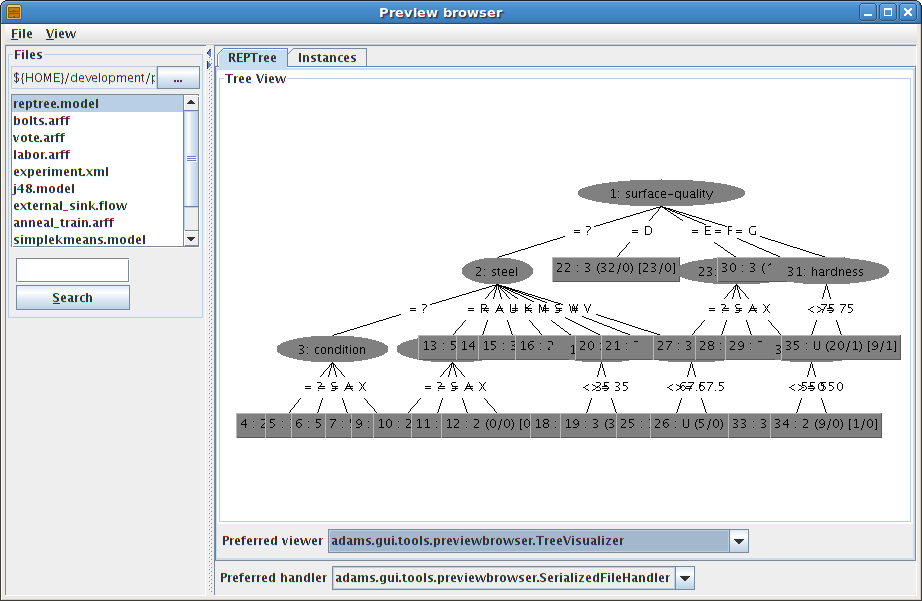
\includegraphics[width=10.0cm]{images/previewbrowser-tree.png}
  \caption{Preview of tree-generating classifier.}
  \label{previewbrowser-tree}
\end{figure}

\begin{figure}[htb]
  \centering
  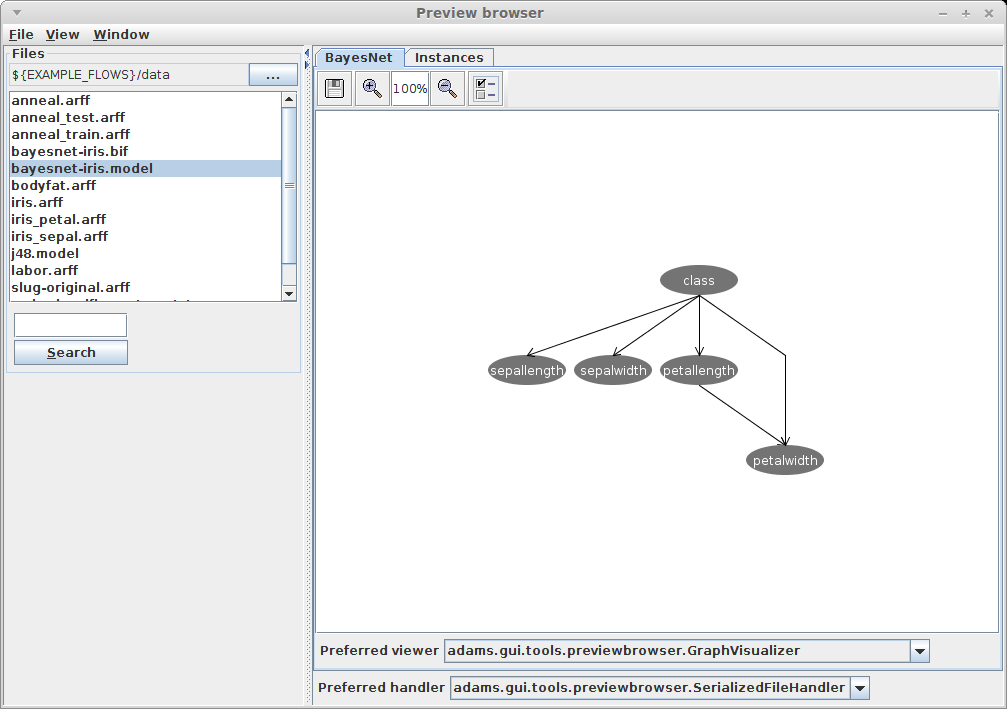
\includegraphics[width=10.0cm]{images/previewbrowser-graph.png}
  \caption{Preview for graph generated by BayesNet classifier.}
  \label{previewbrowser-graph}
\end{figure}


\clearpage
\section{Instance Compare}
Quite often, you generate data with different or tweaked pre-processing 
techniques and you wonder how different the generated data looks like.
The \textit{Instance Compare} visualization allows you to graphically compare
two datasets. You can either compare them row by row, or using a common 
attribute that can be used as unique row identifier.

Figure \ref{instance-compare} shows a comparison of two datasets. Not only
are the two rows overlayed, you also see the absolute difference plotter and
a the correlation coefficient of the two being calculated.

If you don't want to compare all the attributes, you can restrict it to a 
subset, by using the \textit{Att. range} text field. ``first'', ``second'',
``third'', ``last'', ``last\_1'' (last minus 1) and ``last\_2'' (last minus 2)
are accepted indices. All other indices must be 1-based.

\begin{figure}[htb]
  \centering
  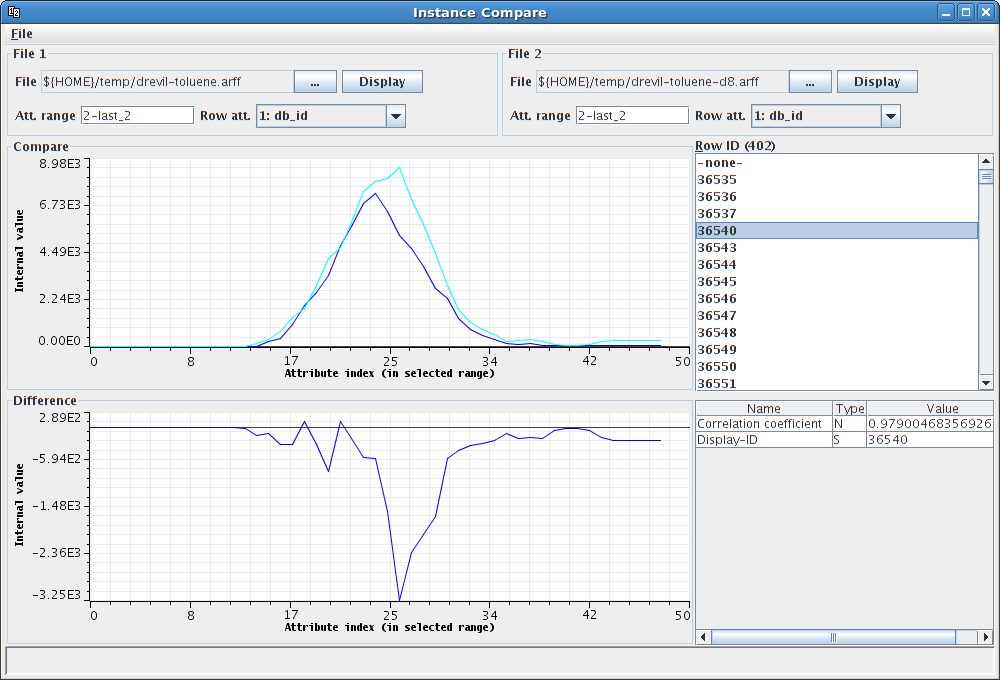
\includegraphics[width=10.0cm]{images/instance-compare.png}
  \caption{Comparing two datasets.}
  \label{instance-compare}
\end{figure}


\clearpage
\section{Instance Explorer}
When generating datasets, it pays to check the generated output in multiple
ways. For instance, whether the data rows generated are actually aligning 
properly. The \textit{Instance Explorer} allows you to select a range of
rows and columns from a dataset (see Figures \ref{instance-explorer_load1}
and \ref{instance-explorer_load2}), which are then displayed in a single
graph.

Figure \ref{instance-explorer_view} shows a subset of the UCI dataset
\textit{waveform-5000}. The top graph of the two is a zoom into the full graph, 
with the bottom graph showing the area that was zoomed into.

\begin{figure}[htb]
  \centering
  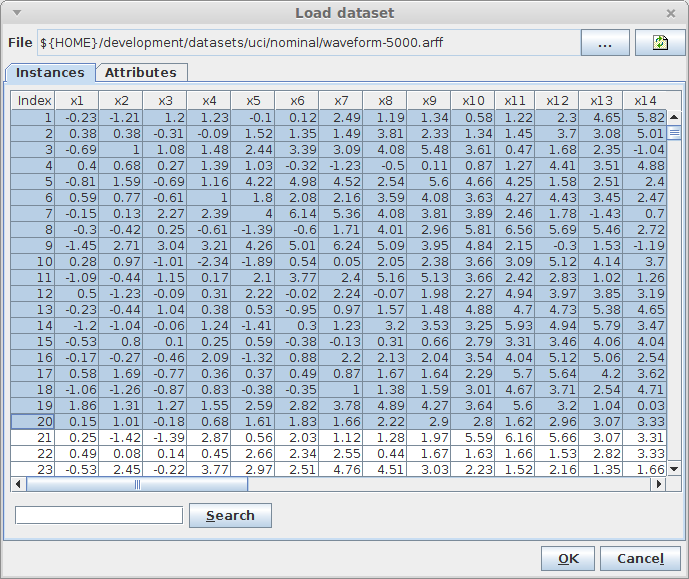
\includegraphics[width=10.0cm]{images/instance-explorer_load1.png}
  \caption{Viewing data in the Instance explorer.}
  \label{instance-explorer_load1}
\end{figure}

\begin{figure}[htb]
  \centering
  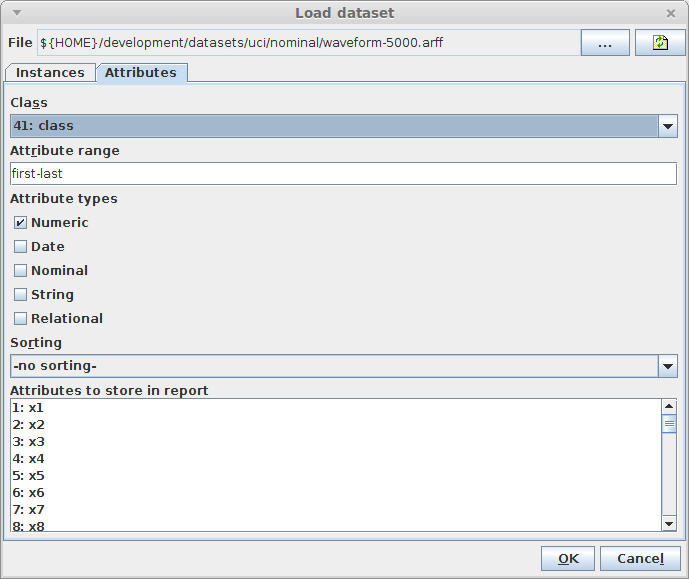
\includegraphics[width=10.0cm]{images/instance-explorer_load2.png}
  \caption{Viewing data in the Instance explorer.}
  \label{instance-explorer_load2}
\end{figure}

\begin{figure}[htb]
  \centering
  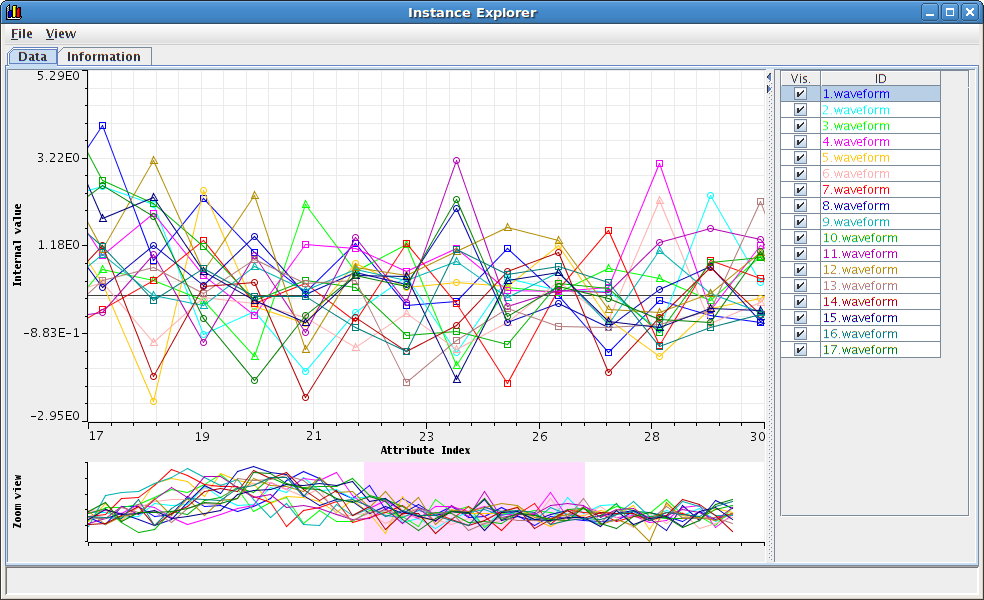
\includegraphics[width=10.0cm]{images/instance-explorer_view.png}
  \caption{Viewing data in the Instance explorer.}
  \label{instance-explorer_view}
\end{figure}

\clearpage
\section{Other visualizations}
Below are some more visualizations, which are available through WEKA and have
been added to the main menu:
\begin{tight_itemize}
  \item \textit{Boundary visualizer} -- visualizes classification boundaries
  \item \textit{Cost curve} -- for re-visualizing a previously displayed cost curve
  \item \textit{Graph visualizer} -- for displaying BayesNet graphs
  \item \textit{Instances plot} -- plots a attributes from a dataset against each other
  \item \textit{Margin curve} -- for re-visualizing a previously displayed margin curve
  \item \textit{Plot attribute vs attribute} -- allows to plot attributes against each other,
  using two user-selected subsets.
  \item \textit{ROC} -- for re-visualizing a previously displayed receiver operator curve
  \item \textit{Tree visualizer} -- for displaying trees graphs (digraph
  format\footnote{\url{https://en.wikipedia.org/wiki/DOT\_\%28graph\_description\_language\%29}{}})
\end{tight_itemize}